% !TeX spellcheck = en_US
\documentclass[12pt,a4paper,openright,oneside]{book}
\usepackage{lineno}
\usepackage[toc , page]{appendix}
\usepackage[top=2.54cm,bottom=3.25cm,left=3.81cm,right=2.54cm]{geometry} %[a4paper, total={6in, 7in}]
\usepackage{amsthm}
\usepackage{fancyhdr}
\usepackage{amsfonts}
\usepackage[dvips]{graphicx}
\usepackage[italian]{babel}
\usepackage[square,sort,comma,numbers]{natbib}
\usepackage{subfigure}
\usepackage{color}
\usepackage{amssymb,amsmath}
\usepackage{amscd}
\usepackage{rotating}
\usepackage{float}
%\usepackage[T1]{fontenc}
\usepackage{afterpage}
\usepackage[dvips]{epsfig}
\usepackage{fancybox}

\usepackage{fancyhdr}

\usepackage{multirow}
\usepackage[utf8]{inputenc}
\usepackage{upgreek}
\usepackage{sidecap}
\usepackage[hidelinks]{hyperref}
\usepackage{physics}
\usepackage{chngpage}
\usepackage{wrapfig}
\usepackage{cancel}
\usepackage{makeidx}
\bibliographystyle{elsarticle-num}
\usepackage{epigraph}
\usepackage{bbold}
%\usepackage[usenames]{color}
\usepackage{tikz, calc}
\usepackage{array}
\usepackage{hyphenat}
\usetikzlibrary{decorations.pathmorphing}
\usepackage{scalerel}

\usepackage{booktabs}
\usepackage{enumitem}
\usepackage{bm}
\usepackage[font=small]{caption}
\usepackage[small]{titlesec}

\usetikzlibrary{decorations.pathmorphing}

%---------------------------------------------------------
\usepackage{mathtools}
\usepackage{multicol}
\usepackage{mathcomp} % simbolo per mille

\usepackage{cancel}

\newcommand{\p}{\partial}
\newcommand{\sx}{\left(}
\newcommand{\dx}{\right)}
\newcommand{\sss}{\left[}
\newcommand{\ddd}{\right]}
\newcommand{\eps}{\varepsilon}
\newcommand{\fii}{\varphi}
\newcommand{\lbar}{\underline}
\newcommand{\spazio}{\mbox{ }}
\newcommand{\complex}{\mathbb{C}}
\newcommand{\seg}{\quad\Rightarrow\quad}

\begin{document}
\begin{titlepage}
\begin{center}
\href{\Grouplink}{
\includegraphics[width=0.15\textwidth]{../logo.png}}\\
\huge{\textbf{Aiuto e Ripetizioni per Materie Scientifiche}}\\
\vspace{25mm}
\hrule
\vspace{2.5mm}
\Huge{\textbf{APPUNTI DI FISICA GENERALE 1}}
\vspace{2.5mm}
\hrule
\vspace{3.5mm}
\Large{Meccanica e Termodinamica}
\\[2.5mm]
\normalsize{
    Bizzi R.\\
    \textcolor[RGB]{\hashcolor}{(\href{\Riccardolink}{\textcolor[RGB]{\hashcolor}{@PaulDiracc}})}
}
\\[5mm]
\href{https://www.esa.int/ESA_Multimedia/Images/2021/04/Dragon_fire}{
    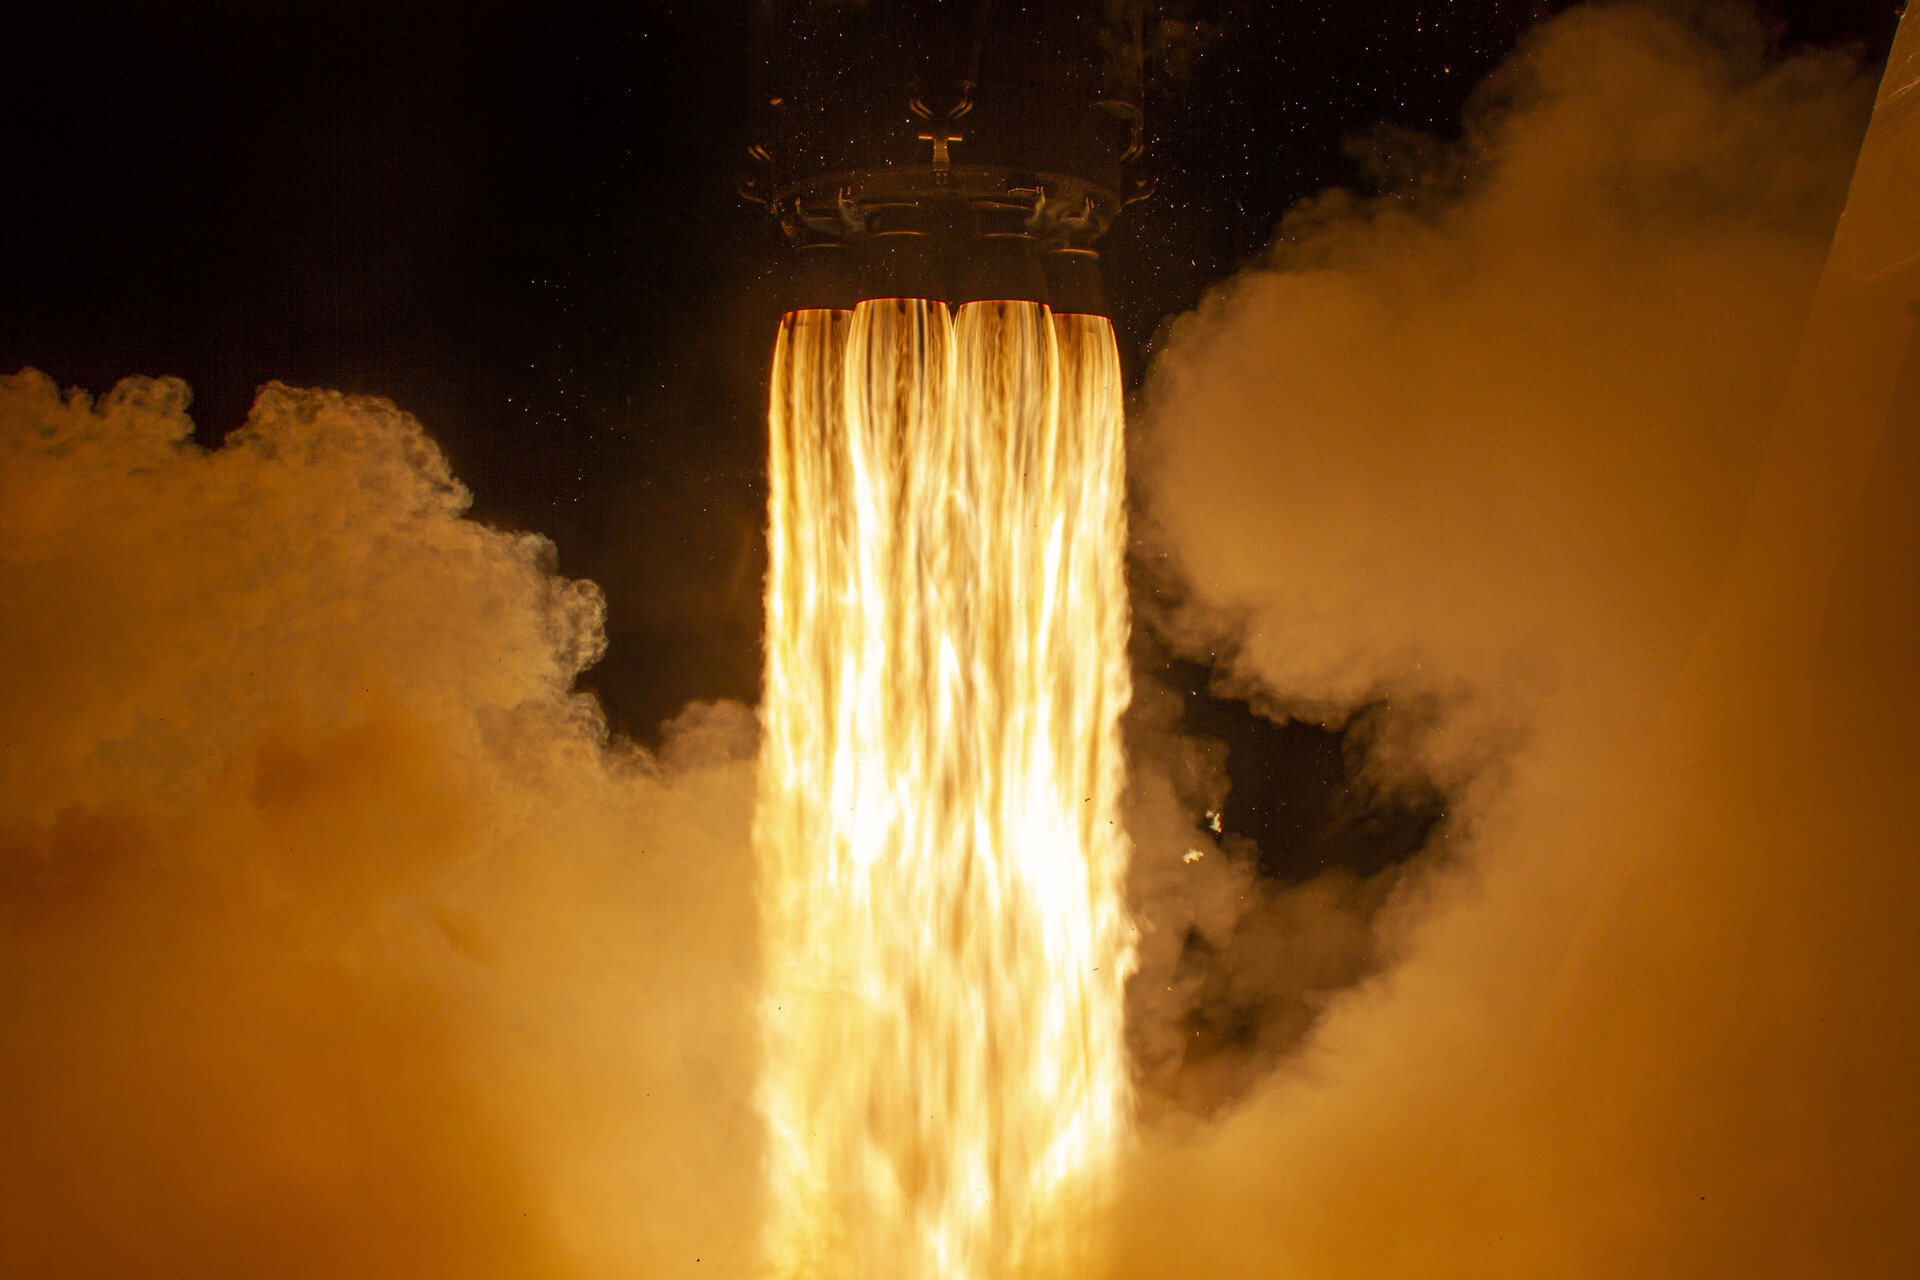
\includegraphics[width=0.9\textwidth]{images/cop.jpg}}
\\[15mm]
\href{\Grouplink}{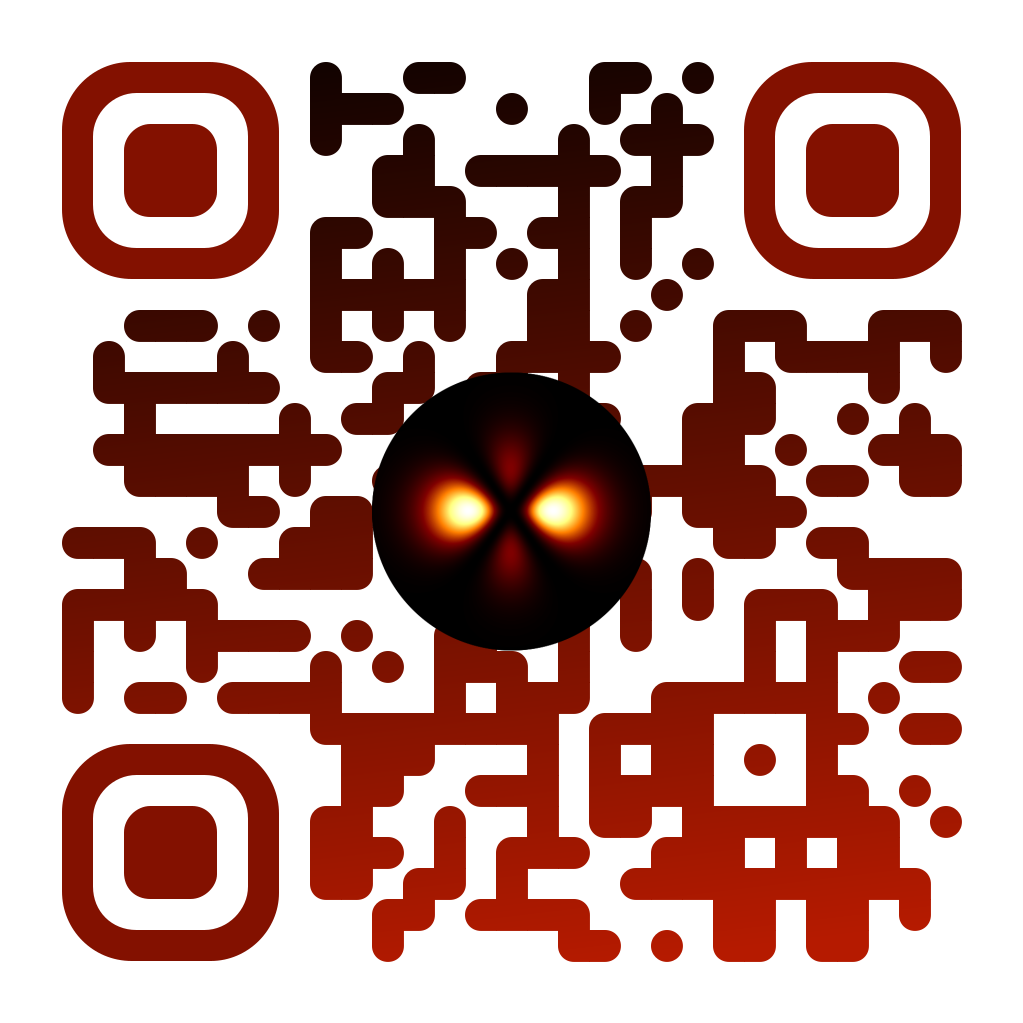
\includegraphics[width=0.15\textwidth]{../QR_group.png}}\qquad
\href{\PayPallink}{
\includegraphics[width=0.14\textwidth]{../QR_PayPal.png}}\qquad
\href{\Riccardolink}{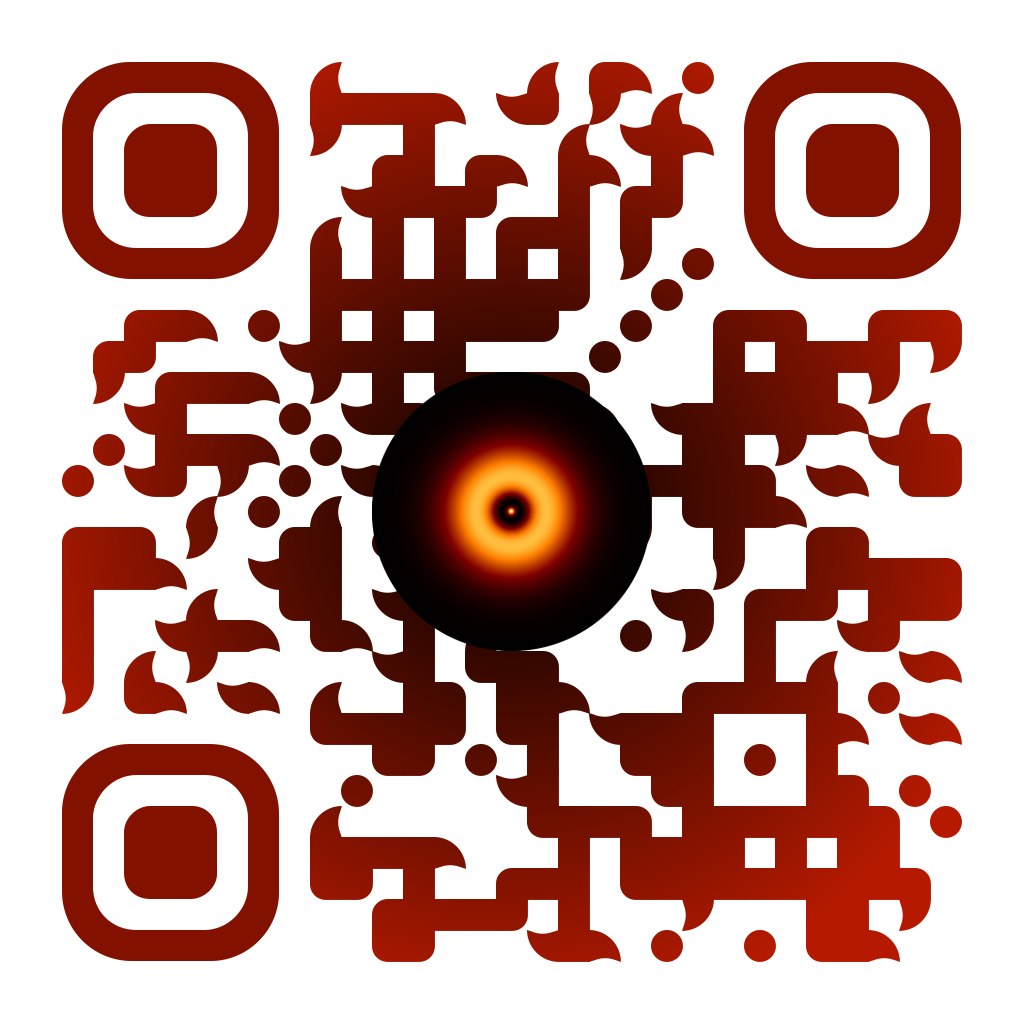
\includegraphics[width=0.15\textwidth]{../QR_me.png}}
\end{center}
\end{titlepage}

\clearpage\null\thispagestyle{empty}\clearpage       % pagina bianca numerata
\tableofcontents %indice

\pagestyle{plain}
\input ./paragraph/1.1-2.9.tex

\input ./paragraph/2.10-2.13.tex

\input ./paragraph/3MotiRelativi.tex

\begin{thebibliography}{999}
\addcontentsline{toc}{chapter}{Bibliografia}
%%%esempio bibliografia%%%

\bibitem{cit1}
P. Mazzoldi, M. Nigro, C. Voci - Fisica (Volume 1)
\bibitem{cit2}
https://elearning.uniroma1.it/pluginfile.php/996072/course/summary/physics.jpg
\end{thebibliography}


\end{document}